% Define important features for the document
\documentclass[12pt,oneside]{article}
\setlength{\parindent}{0pt}
\setlength{\parskip}{4pt}

% Import packages
\usepackage[margin = 1in]{geometry}
\usepackage{amsfonts, amsmath, amssymb, amsthm, calc, centernot, color, csquotes, dsfont, enumitem, environ, fancyhdr, fontawesome5, graphicx, hyperref, marvosym, mathrsfs, mathtools, tcolorbox, titlesec}
\usepackage[flushmargin,hang]{footmisc}
\tcbuselibrary{breakable}

% Define toggles
\newif\ifsolutions
\solutionstrue % Toggle for instructor version
% \solutionsfalse % Toggle for student version

% Define size and spacing of section and subsection
\titleformat{\section}
  {\normalfont\large\bfseries}
  {\thesection}{1em}{}
\titleformat{\subsection}
  {\normalfont\normalsize\bfseries}
  {\thesubsection}{1em}{}
\titlespacing*{\section}{0pt}{6pt}{6pt} % ({left}{before}{after})
\titlespacing*{\subsection}{0pt}{6pt}{6pt} % ({left}{before}{after})

% Define commands
\newcommand{\indep}{\perp\!\!\!\perp}
\newcommand{\notindep}{\mathrel{\not\!\perp\!\!\!\perp}}
\newcommand{\E}{\mathbb{E}}
\newcommand{\Var}{\text{Var}}
\newcommand{\Cov}{\text{Cov}}
\newcommand{\Corr}{\text{Corr}}
\newcommand{\SD}{\text{SD}}
\newcommand{\SE}{\text{SE}}
\newcommand{\Bias}{\text{Bias}}
\newcommand{\MSE}{\text{MSE}}
\newcommand{\Risk}{\text{Risk}}
\newcommand{\Like}{\mathcal{L}}
\newcommand{\boot}{\text{boot}}
\newcommand{\strat}{\text{strat}}
\newcommand{\supp}{\text{supp}}
\newcommand{\MLE}{\text{MLE}}
\newcommand{\MoM}{\text{MoM}}
\newcommand{\MOM}{\text{MOM}}
\newcommand{\OLS}{\text{OLS}}
\newcommand{\LS}{\text{LS}}
\newcommand{\MAP}{\text{MAP}}
\newcommand{\MAE}{\text{MAE}}
\newcommand{\LP}{\text{LP}}
\newcommand{\HT}{\text{HT}}
\newcommand{\JS}{\text{JS}}
\newcommand{\RB}{\text{RB}}
\newcommand{\UB}{\text{UB}}
\newcommand{\DIM}{\text{DIM}}
\newcommand{\PATE}{\text{PATE}}
\newcommand{\SATE}{\text{SATE}}
\newcommand{\VIF}{\text{VIF}}
\newcommand{\GVIF}{\text{GVIF}}
\newcommand{\AIC}{\text{AIC}}
\newcommand{\BIC}{\text{BIC}}
\newcommand{\LASSO}{\text{LASSO}}
\newcommand{\PSS}{\text{PSS}}
\newcommand{\CV}{\text{CV}}
\newcommand{\logit}{\text{logit}}
\newcommand{\odds}{\text{odds}}
\newcommand{\OR}{\text{OR}}
\newcommand{\N}{\mathcal{N}}
\newcommand{\Bern}{\text{Bern}}
\newcommand{\Bin}{\text{Bin}}
\newcommand{\Beta}{\text{Beta}}
\newcommand{\Gam}{\text{Gamma}}
\newcommand{\Expo}{\text{Expo}}
\newcommand{\Pois}{\text{Pois}}
\newcommand{\Unif}{\text{Unif}}
\newcommand{\DUnif}{\text{DUnif}}
\newcommand{\Geom}{\text{Geom}}
\newcommand{\FS}{\text{FS}}
\newcommand{\NBin}{\text{NBin}}
\newcommand{\HGeom}{\text{HGeom}}
\newcommand{\Mult}{\text{Mult}}
\newcommand{\MVN}{\text{MVN}}
\newcommand{\IG}{\text{IG}}
\newcommand{\Tweedie}{\text{Tweedie}}
\newcommand{\simiid}{\overset{\text{i.i.d.}}{\sim}}
\newcommand{\simind}{\overset{\text{ind.}}{\sim}}
\newcommand{\simnull}{\overset{H_0}{\sim}}
\newcommand{\simapprox}{\overset{\cdot}{\sim}}
\newcommand{\R}{\mathbb{R}}
\newcommand{\Z}{\mathbb{Z}}
\newcommand{\Q}{\mathbb{Q}}
\newcommand{\C}{\mathbb{C}}
\newcommand{\I}{\mathbb{I}}
\newcommand{\indic}{\mathds{1}}
\newcommand{\iid}{\text{i.i.d.}}
\newcommand{\Ind}{\text{Ind}}
\newcommand{\SSq}{\text{SSq}}
\newcommand{\trace}{\text{trace}}
\newcommand{\rank}{\text{rank}}
\newcommand{\diag}{\text{diag}}
\newcommand{\adj}{\text{adj}}
\newcommand{\SSE}{\text{SSE}}
\newcommand{\SST}{\text{SST}}
\newcommand{\SSR}{\text{SSR}}
\newcommand{\GLS}{\text{GLS}}
\newcommand{\ti}{\text{time}}
\newcommand{\outcome}{\text{outcome}}
\newcommand{\exposure}{\text{exposure}}
\newcommand{\NA}{\text{NA}}
\newcommand{\cp}{\text{cp}}
\newcommand{\tip}{\textbf{\faLightbulb}: }
\newcommand{\warning}{\textbf{\Biohazard}: }
\newcommand{\blank}[1][4cm]{\underline{\hspace{#1}}}

% Define theorem-style environment (italic body, bold header)
\newtheorem{theorem}{Theorem}
\newtheorem{lemma}{Lemma}
\newtheorem{proposition}{Proposition}
\newtheorem{corollary}{Corollary}

% Define definition-style environment (upright body, bold header)
\theoremstyle{definition}
\newtheorem{definition}{Definition}
\newtheorem{example}{Example}
\newtheorem{problem}{\faPen \ Problem}
\newtheorem{concept}{\faPen \ Concept Checker}
\newtheorem{challenge}{\faFire \ Challenge}
\newtheorem{activity}{\faDiceThree \ Activity}

% Define idea-style environment (unnumbered definition)
\newtheorem*{idea}{Idea}

% Define remark-style environment (upright body, italic header)
\theoremstyle{remark}
\newtheorem{remark}{Remark}

% Define environment for solution box
\newsavebox{\solutioncontentbox}
\NewEnviron{solutionbox}[1][Solution]{
  \sbox{\solutioncontentbox}{
    \begin{minipage}{\dimexpr\linewidth-2\fboxsep\relax}
      \BODY
    \end{minipage}
  }
  \ifsolutions
    \begin{tcolorbox}[
      title=#1,
      colback=gray!5,
      colframe=black,
      breakable
    ]
      \BODY
    \end{tcolorbox}
  \else
    \begin{tcolorbox}[
      title=#1,
      colback=white,
      colframe=black,
      breakable,
      height=\dimexpr\ht\solutioncontentbox+\dp\solutioncontentbox+1cm\relax
    ]
    \end{tcolorbox}
  \fi
}

% Begin document
\begin{document}
\pagestyle{fancy}
\fancyhead[L]{STAT 110: Introduction to Probability}
\fancyhead[R]{Fall 2026}
\begin{center}
\bf \Large
Section 2: Conditional Probability \\[0.5em]
\normalsize
Avery Kim (\href{mailto:averykim@college.harvard.edu}{\texttt{averykim@college.harvard.edu}}), \\[0.2em]
Ricky Truong (\href{mailto:rickytruong@college.harvard.edu}{\texttt{rickytruong@college.harvard.edu}})
\end{center}

% Section: Introduction
\section{Introduction}

\subsection{Logistics}

Welcome! The goal of our weekly section is to review content from lecture, with emphasis on big-picture intuition, mathematical derivation, and hands-on practice.

Specifically, we aim for section to be interactive, well-paced, inclusive, and fun! Please do not hesitate to reach out if you have any questions/feedback!

\subsection{Office Hours}

$\bullet$ See the Google Calendar for the most accurate information!

\subsection{Attendance}

$\bullet$ \href{https://bit.ly/stat110harvard}{\texttt{bit.ly/stat110harvard}}

% Section: Non-Naive Probability
\section{Non-Naive Probability}

\begin{idea}
We'll now generalize probability to the \textit{non-naive case}, which allows for much more flexibility. As we'll see, all the important properties of probability can be built from simply two axioms.
\end{idea}

\begin{definition}[Axioms of probability]
A \textit{probability space} consists of a \textit{sample space} $S$ and a \textit{probability function} $P$, which takes an \textit{event} $A \subseteq S$ as input and returns $P(A)$, a real number between $0$ and $1$, as output. The function $P$ must satisfy the following axioms: 

\[P(\emptyset) = 0,\] \[P(S) = 1,\] and if $A_1, A_2, \ldots$ are disjoint events, then \[P \left( \cup_{i = 1}^{\infty} A_i \right) = \sum_{i = 1}^{\infty} P(A_i).\]
\end{definition}

\begin{definition}[Properties of probability]
Informally, \textit{probability} is a measure of how likely an event is, bounded from $0$ to $1$.\footnote{In the \textit{Frequentist} paradigm, probability can be viewed as long-term frequency. E.g., the probability of an ace is $p = \frac{1}{13}$, so in the long run, we expect 1 ace for every 13 cards.} With the axioms above, probability satisfies the following properties:

\[P(A^c) = 1 - P(A),\] \[P(A \cup B) = P(A) + P(B) - P(A \cap B),\] and \[A \subseteq B \implies P(A) \leq P(B).\]

$\bullet$ \tip The complement is useful for finding the event of \enquote{at least} something.
\end{definition}

\begin{concept}
If I roll a fair 6-sided die three times, what is the probability that I land 5 or higher at least once?
\end{concept}

\begin{solutionbox}
Let $A$ be the event that I land 5 or higher at least once. We want $P(A)$, but since this is the event of \enquote{at least} something, it's easier to find the complement. (Notice I can roll 5 on only the first roll, 5 on only the second roll, 5 on the first two rolls, and so on, so the situation quickly gets complicated!)

\[
\begin{aligned}
P(A) &= 1 - P(A^c) && \text{by complement rule} \\
&= 1 - (4/6)^3 && \text{since we can roll 1, 2, 3, or 4} \\
&= 19/27 && \text{by simplifying}
\end{aligned}
\]
\end{solutionbox}

\begin{center}
  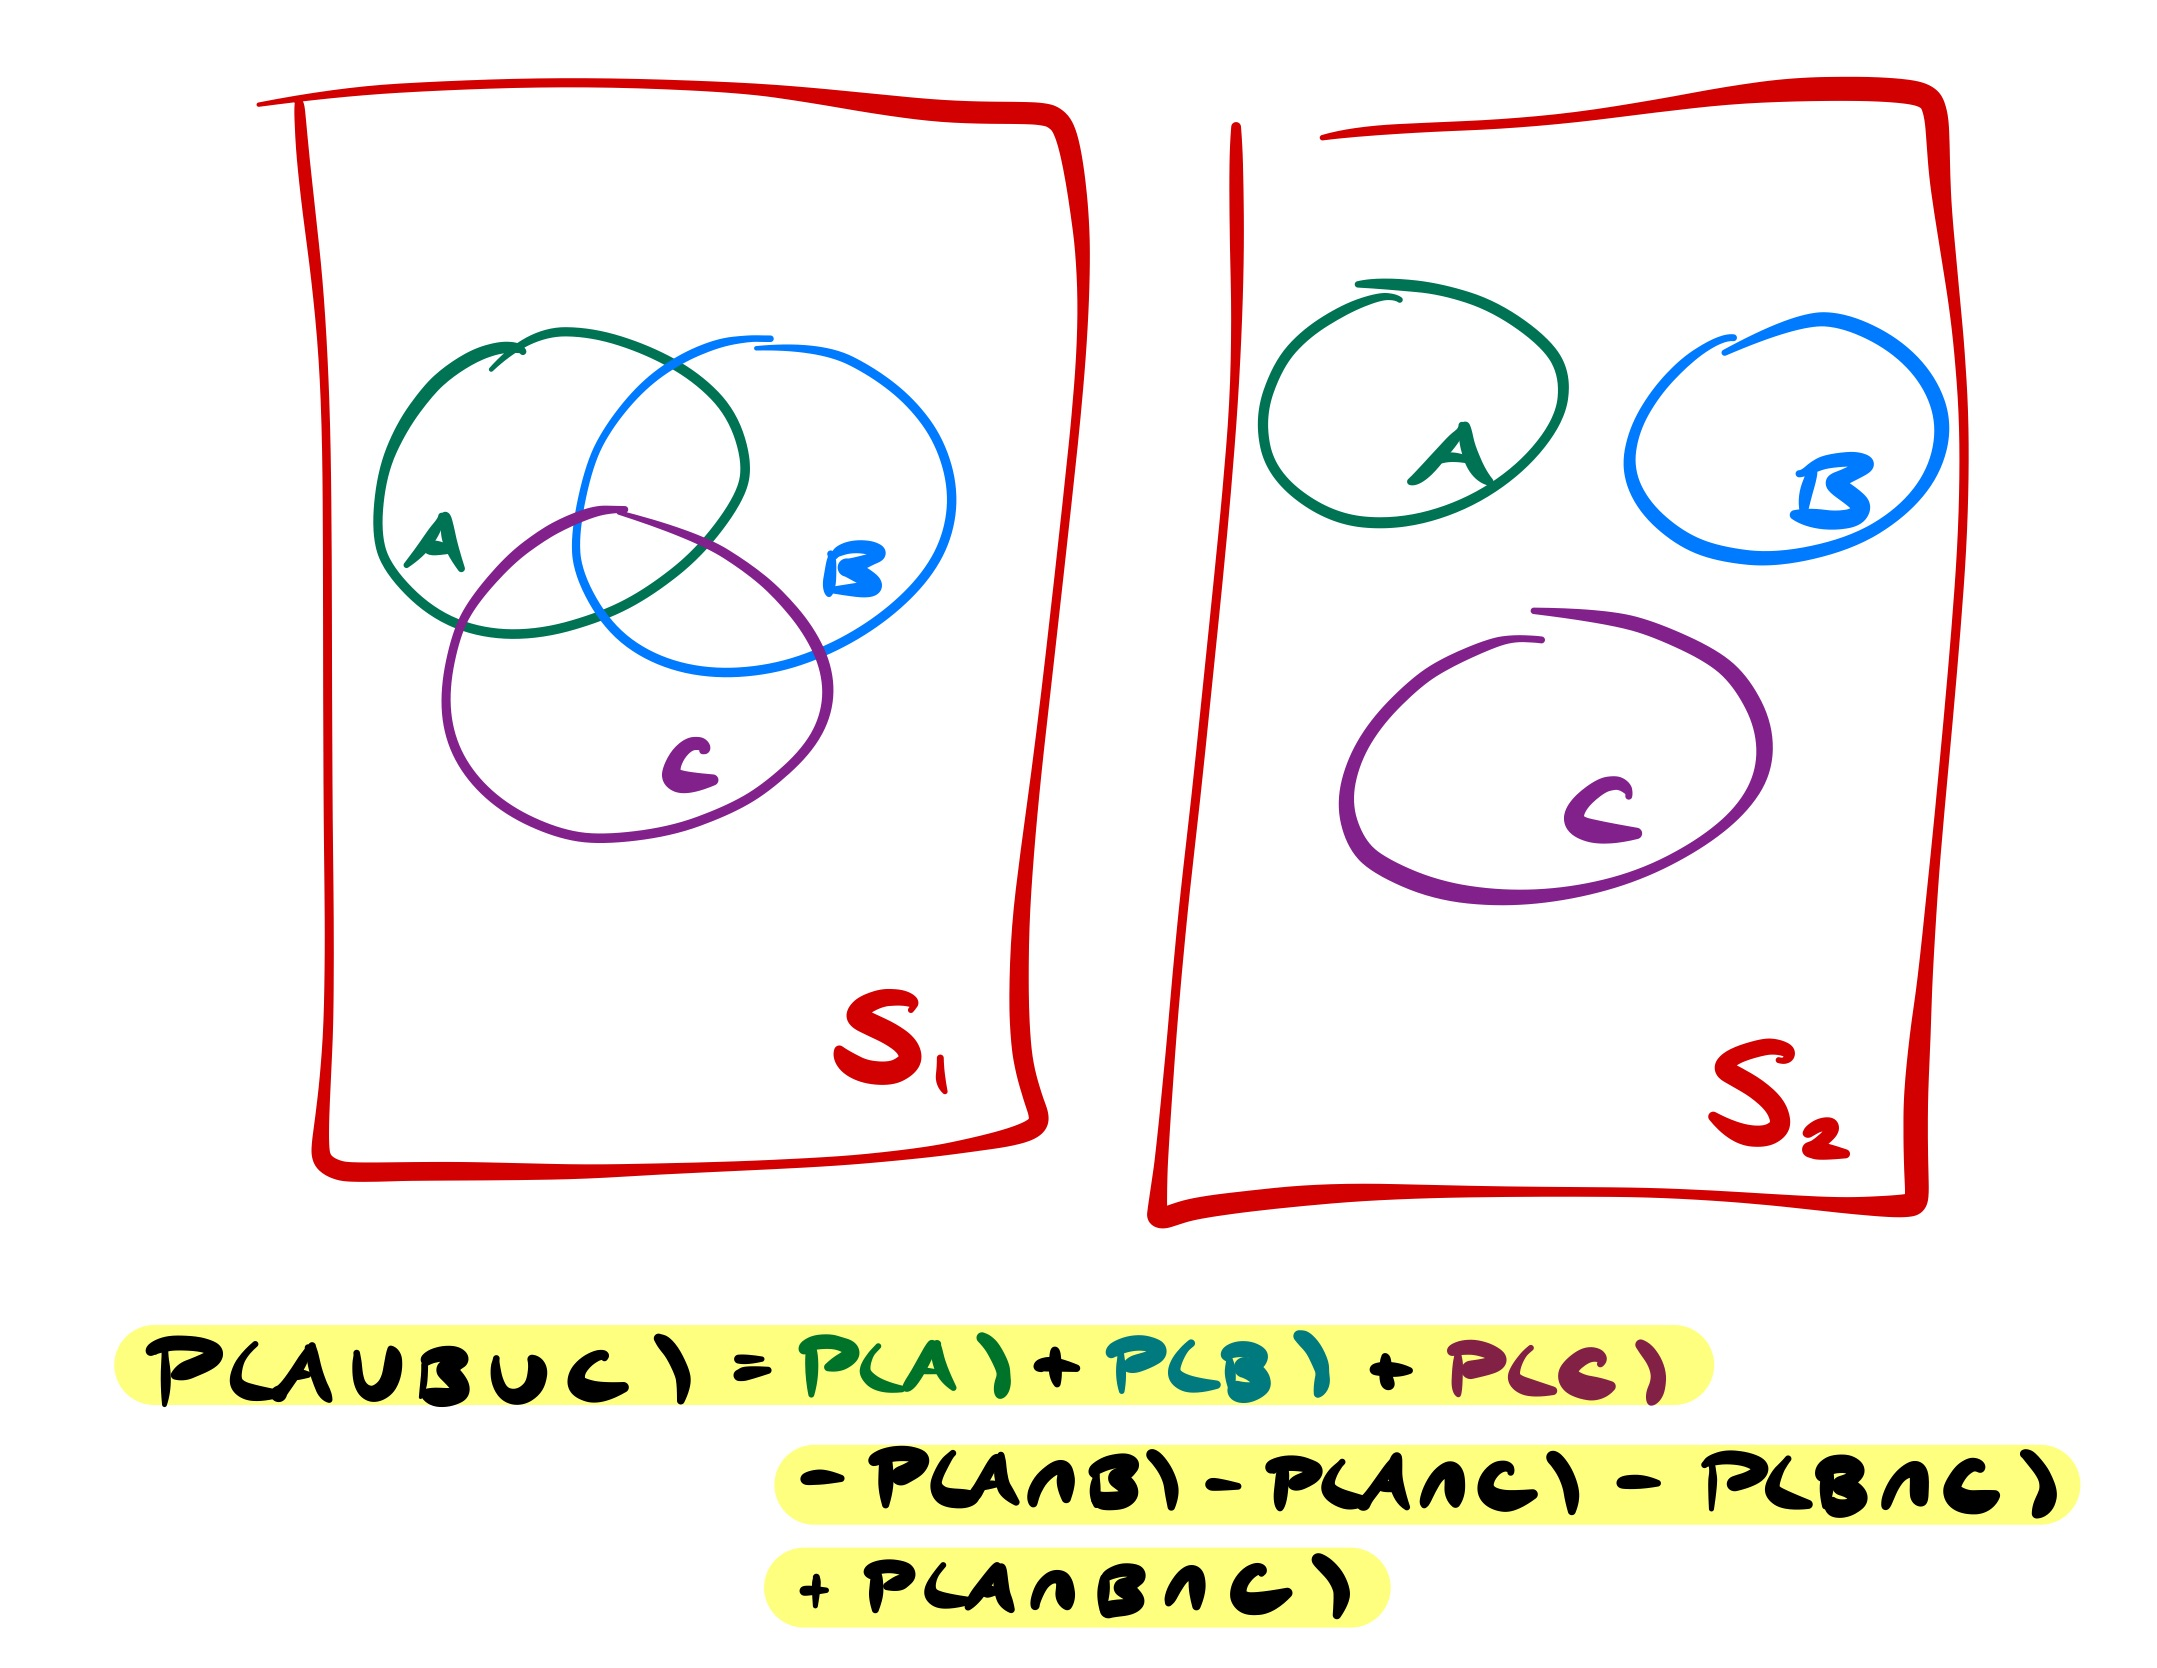
\includegraphics[width=0.5\textwidth]{stat110_section2_figure1.jpg}\\{\footnotesize FIGURE 1: The sample space with Venn diagrams illustrating PIE for 3 events.}
\end{center}

\begin{definition}[Principle of inclusion-exclusion (PIE)]
A useful tool for finding the probability of \textit{unions} of events.

$\bullet$ Informally, \[P(\text{union of many events}) = \text{singles} - \text{doubles} + \text{triples} - \text{quadruples} + \cdots.\]

$\bullet$ Formally, \[P(A_1 \cup \cdots \cup A_n) = \sum_{i} P(A_i) - \sum_{i < j} P(A_i \cap A_j) + \sum_{i < j < k} P(A_i \cap A_j \cap A_k) - \cdots + (-1)^{n + 1} P(A_1 \cap \cdots \cap A_n).\]

$\bullet$ E.g., with 3 events, \[P(A \cup B \cup C) = P(A) + P(B) + P(C) - P(A \cap B) - P(A \cap C) - P(B \cap C) + P(A \cap B \cap C).\]
\end{definition}

\begin{definition}[Symmetry]
Some problems can be greatly simplified if they contain \textit{symmetry} such that \textit{outcomes are equally likely}.

$\bullet$ E.g., if $P(A_1) = P(A_i)$ for all $i$, $P(A_1 \cap A_2) = P(A_i \cap A_j)$ for all $i \neq j$, and so on, then PIE simplifies to $P(A_1 \cup \ldots \cup A_n) = \binom{n}{1} P(A_1) - \binom{n}{2} P(A_1 \cap A_2) + \binom{n}{3} P(A_1 \cap A_2 \cap A_3) - \ldots + (-1)^{n + 1} P(A_1 \cap \ldots \cap A_n)$.
\end{definition}

\begin{concept}
With 3 events, what is $P(A \cup B \cup C)$ if there is no overlap between $A$, $B$, and $C$ (i.e., if $P(A \cap B) = P(B \cap C) = P(A \cap C) = P(A \cap B \cap C) = 0$)?
\end{concept}

\begin{solutionbox}
If there is no overlap between $A$, $B$, and $C$, then $P(A \cup B \cup C) = P(A) + P(B) + P(C)$ (i.e., the sum of the marginal probabilities). PIE adds/subtracts additional terms to adjust for overlap, but in this simple case, there is none!
\end{solutionbox}

% Section: Joint, Marginal, and Conditional Probabilities
\section{Joint, Marginal, and Conditional Probabilities}

\begin{idea}
We'll define some important terms to introduce the idea of \textit{conditional probability}, one of the most important concepts in all of statistics. With it, we'll expand our toolkit to calculate various types of probabilities (conditional, joint, marginal, etc.).
\end{idea}

\begin{definition}[Joint probability]
$P(A \cap B) = P(A, B)$ is the \textit{joint probability} of $A$ and $B$.

$\bullet$ Importantly, $P(A \cap B) = P(B \cap A)$.

$\bullet$ \tip We can treat $A \cap B$ (or any union or intersection) as \textit{one} event! Thus, all the previous rules carry over. E.g., $P((A \cap B)^c) = 1 - P(A \cap B)$ by complement rule.
\end{definition}

\begin{definition}[Marginal probability]
$P(A)$ is the \textit{marginal probability} of $A$ (i.e., \enquote{by itself}).

$\bullet$ Equivalently, this is the \textit{unconditional} or \textit{prior} probability.
\end{definition}

\begin{center}
  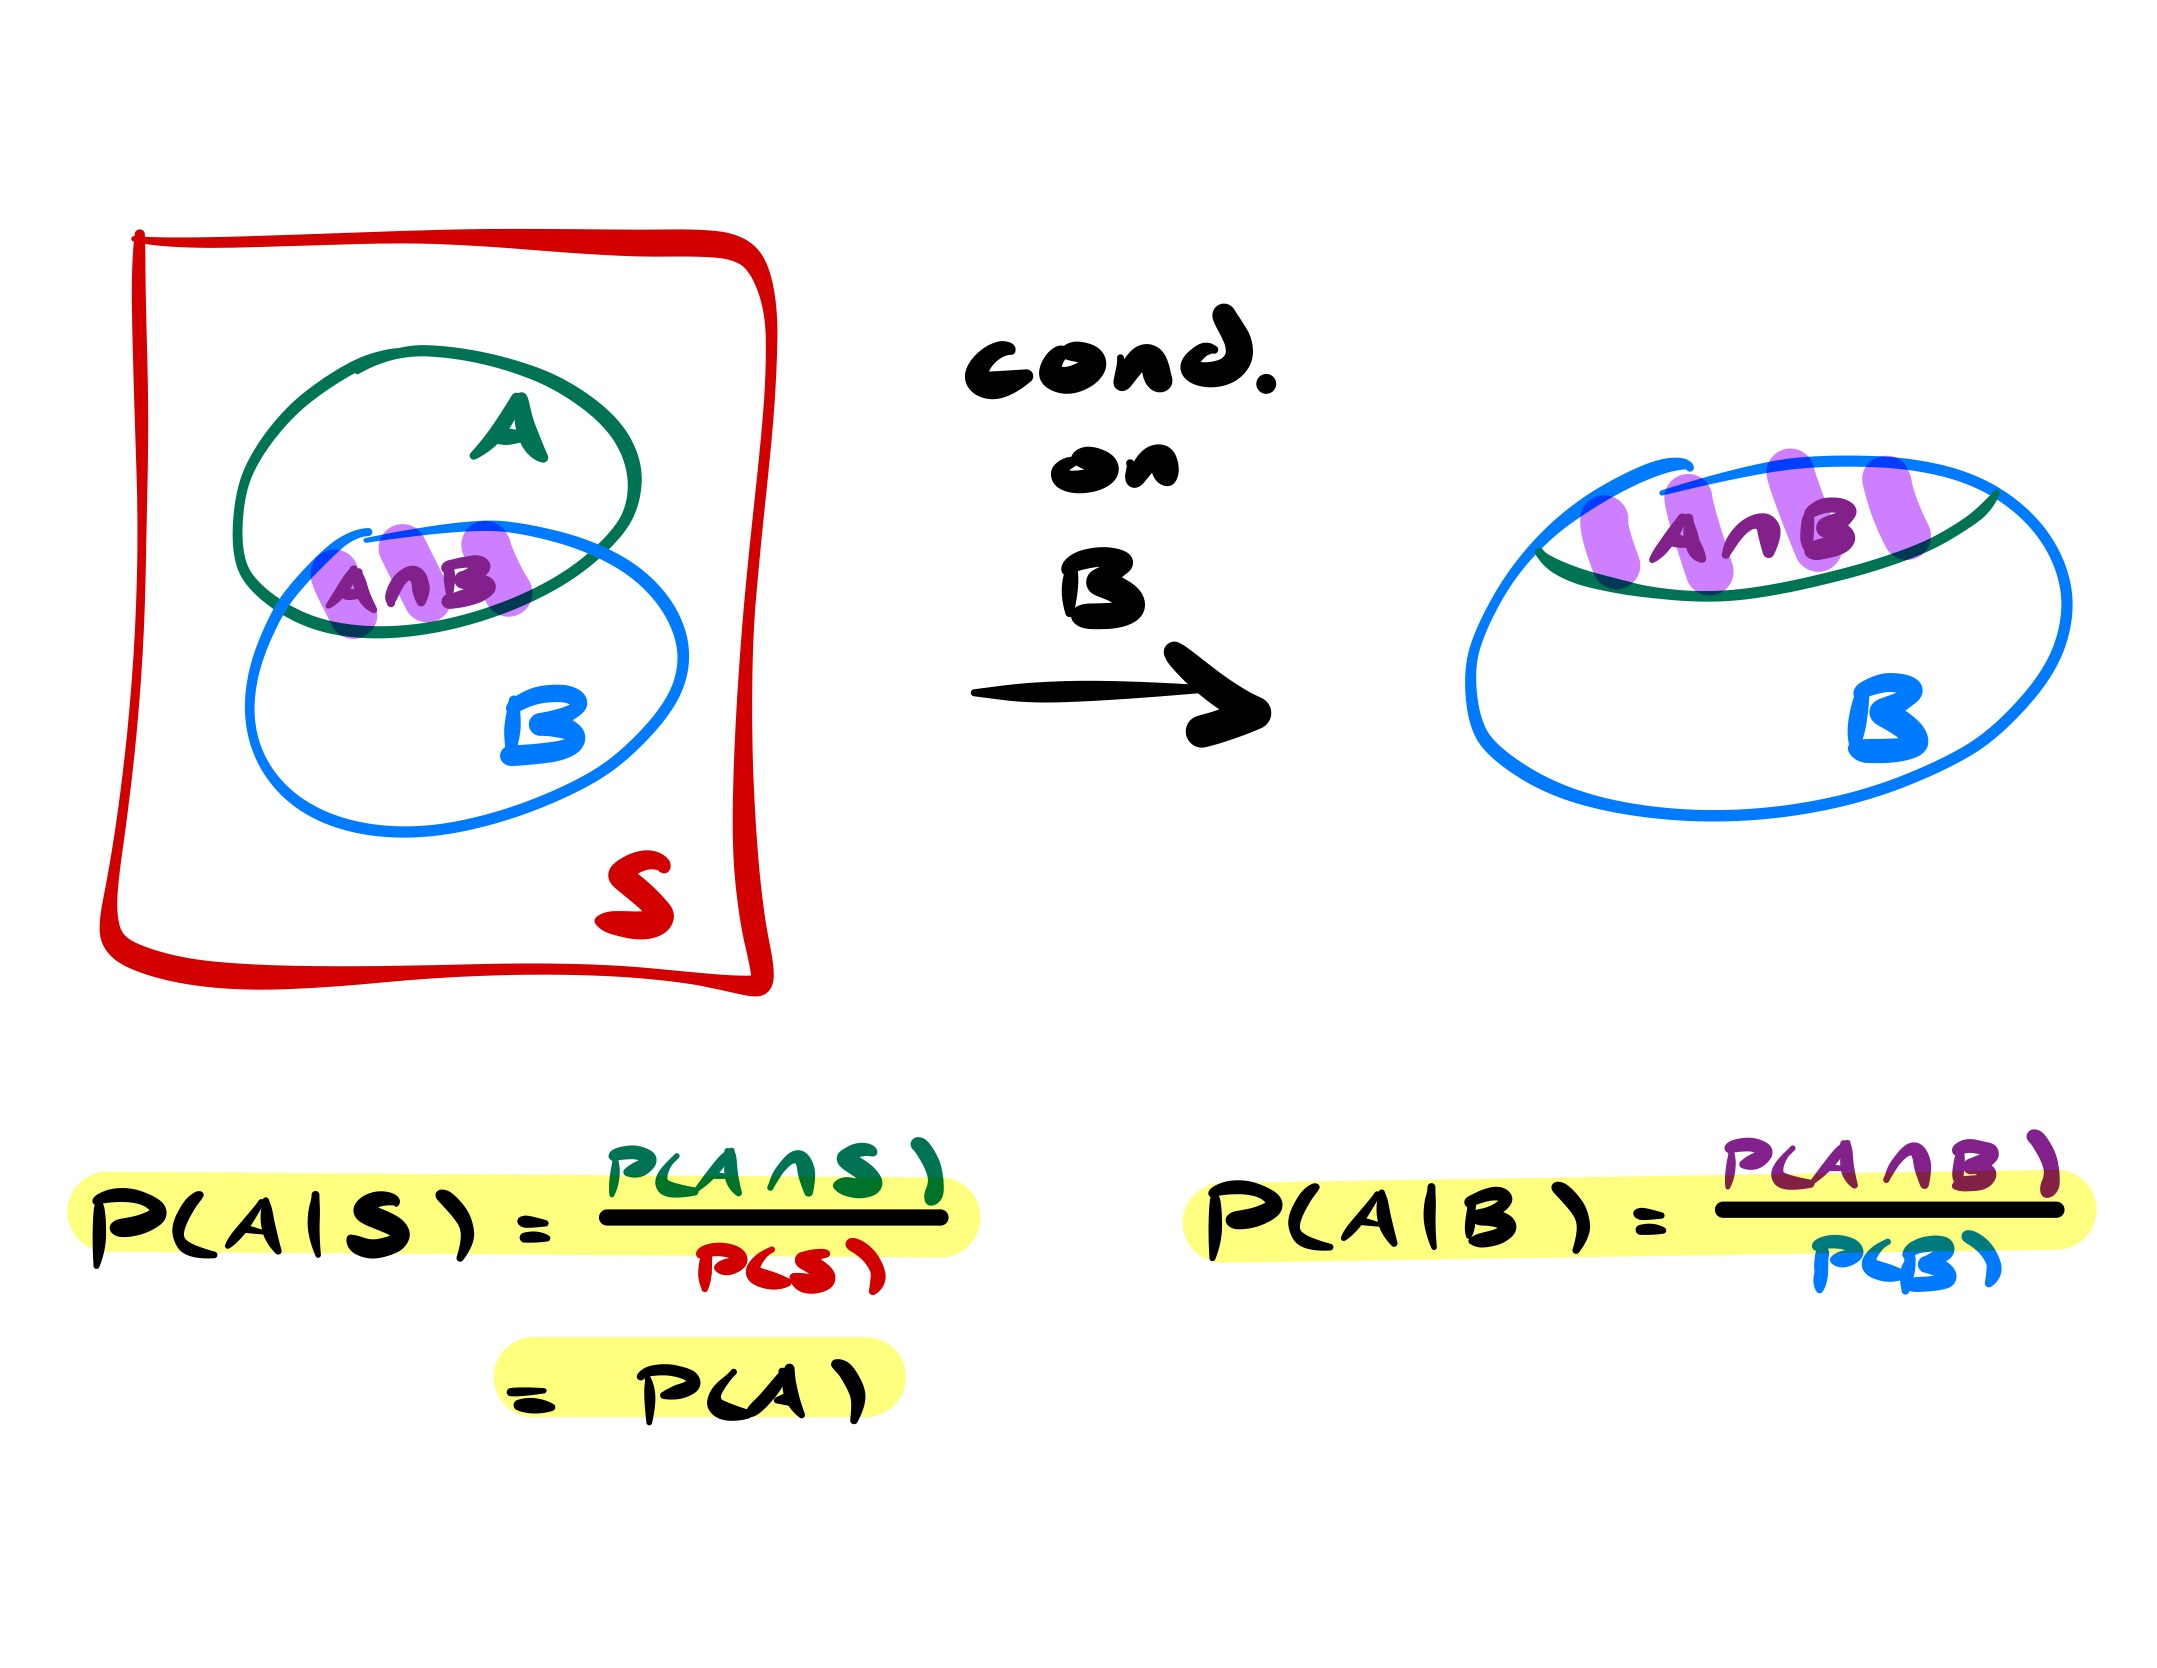
\includegraphics[width=0.5\textwidth]{stat110_section2_figure2.jpg}\\{\footnotesize FIGURE 2: The sample space before and after conditioning.}
\end{center}

\begin{center}
  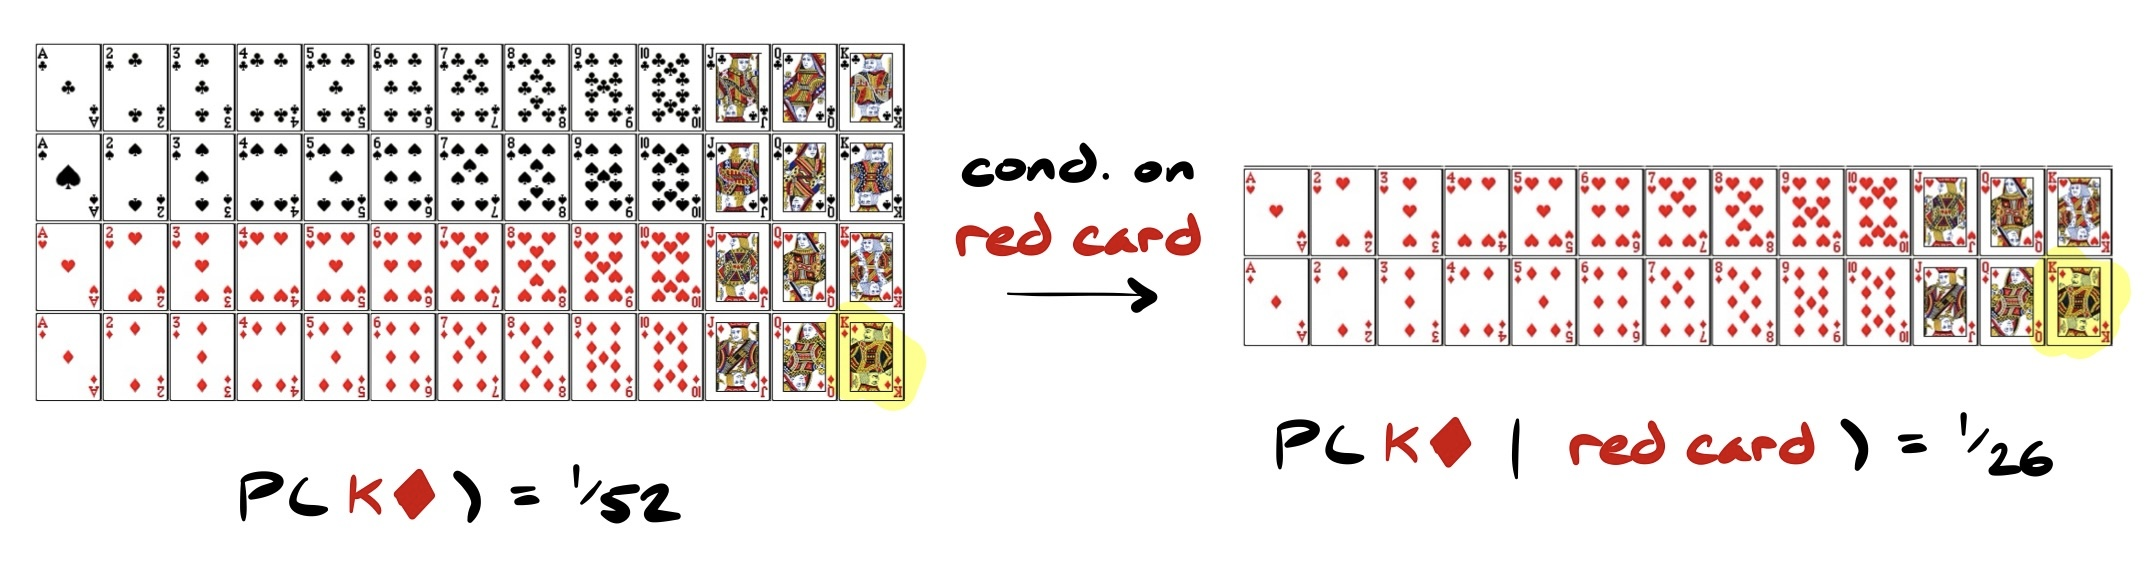
\includegraphics[width=0.75\textwidth]{stat110_section2_figure3.jpg}\\
  {\footnotesize FIGURE 3: A standard deck of 52 playing cards shrunk down to only the 26 red cards.}
\end{center}

\begin{definition}[Conditional probability]
\[P(A \mid B) = \frac{P(A \cap B)}{P(B)}\] is the \textit{conditional probability} of $A$ given that $B$ occurred, where $P(B) > 0$.

$\bullet$ When we \textit{condition} on $B$, we reduce the sample space to the area where $B$ occurs (i.e., we divide by $P(B)$). Within this new space, the area where $A$ occurs is the \textit{intersection} of $A$ and $B$ (i.e., we calculate $P(A \cap B)$). This is illustrated in Figure 2 and Figure 3.

$\bullet$ \warning In general, $P(A \mid B) \neq P(B \mid A)$!

$\bullet$ \tip All conditional probabilities \textit{are} probabilities, and all probabilities \textit{are} conditional probabilities (implicitly conditioning on $S$). Thus, all the previous rules carry over. E.g., $P(A^c \mid B) = 1 - P(A \mid B)$ by complement rule.
\end{definition}

\begin{concept}
Rearrange the definition of conditional probability to get two formulas for $P(A \cap B)$. How do these connect to the multiplication rule?
\end{concept}

\begin{solutionbox}
$P(A \mid B) = \frac{P(A \cap B)}{P(B)} \implies P(A \cap B) = P(B) P(A \mid B)$. $P(B \mid A) = \frac{P(B \cap A)}{P(A)} \implies P(B \cap A) = P(A \cap B) = P(A) P(B \mid A)$. Using the same logic as the multiplication rule, we can imagine two tree diagrams. First, $A$ happens, and then $B$ happens (given that $A$ happened). Equivalently, $B$ happens, and then $A$ happens (given that $B$ happened).
\end{solutionbox}

\begin{concept}
Using the multiplication rule, what is a formula for $P(A_1, \ldots, A_n)$? How many formulas are there in total?
\end{concept}

\begin{solutionbox}
$P(A_1, \ldots, A_n) = P(A_1) P(A_2 \mid A_1) P(A_3 \mid A_1, A_2) \cdots P(A_n \mid A_1, \ldots, A_{n - 1})$. There are $n!$ total formulas (since we could've started with $P(A_i)$ for any of the $n$ available $i$, followed by $P(A_j \mid A_i)$ for any of the $n - 1$ remaining $j$, and so on).
\end{solutionbox}

\begin{definition}[Bayes' Rule]
\[P(A \mid B) = \frac{P(B \mid A) P(A)}{P(B)},\] where $P(B) > 0$.

$\bullet$ \tip Often, we want to find $P(A \mid B)$ but are given $P(B \mid A)$. This is where Bayes' Rule is useful!
\end{definition}

\begin{concept}
Derive Bayes' Rule using the definition of conditional probability.
\end{concept}

\begin{solutionbox}
\[
\begin{aligned}
P(A \mid B) &= \frac{P(A \cap B)}{P(B)} && \text{by definition of conditional probability} \\
&= \frac{P(A) P(B \mid A)}{P(B)} && \text{since $P(A \cap B) = P(A) P(B \mid A)$}
\end{aligned}
\]
\end{solutionbox}

\begin{center}
  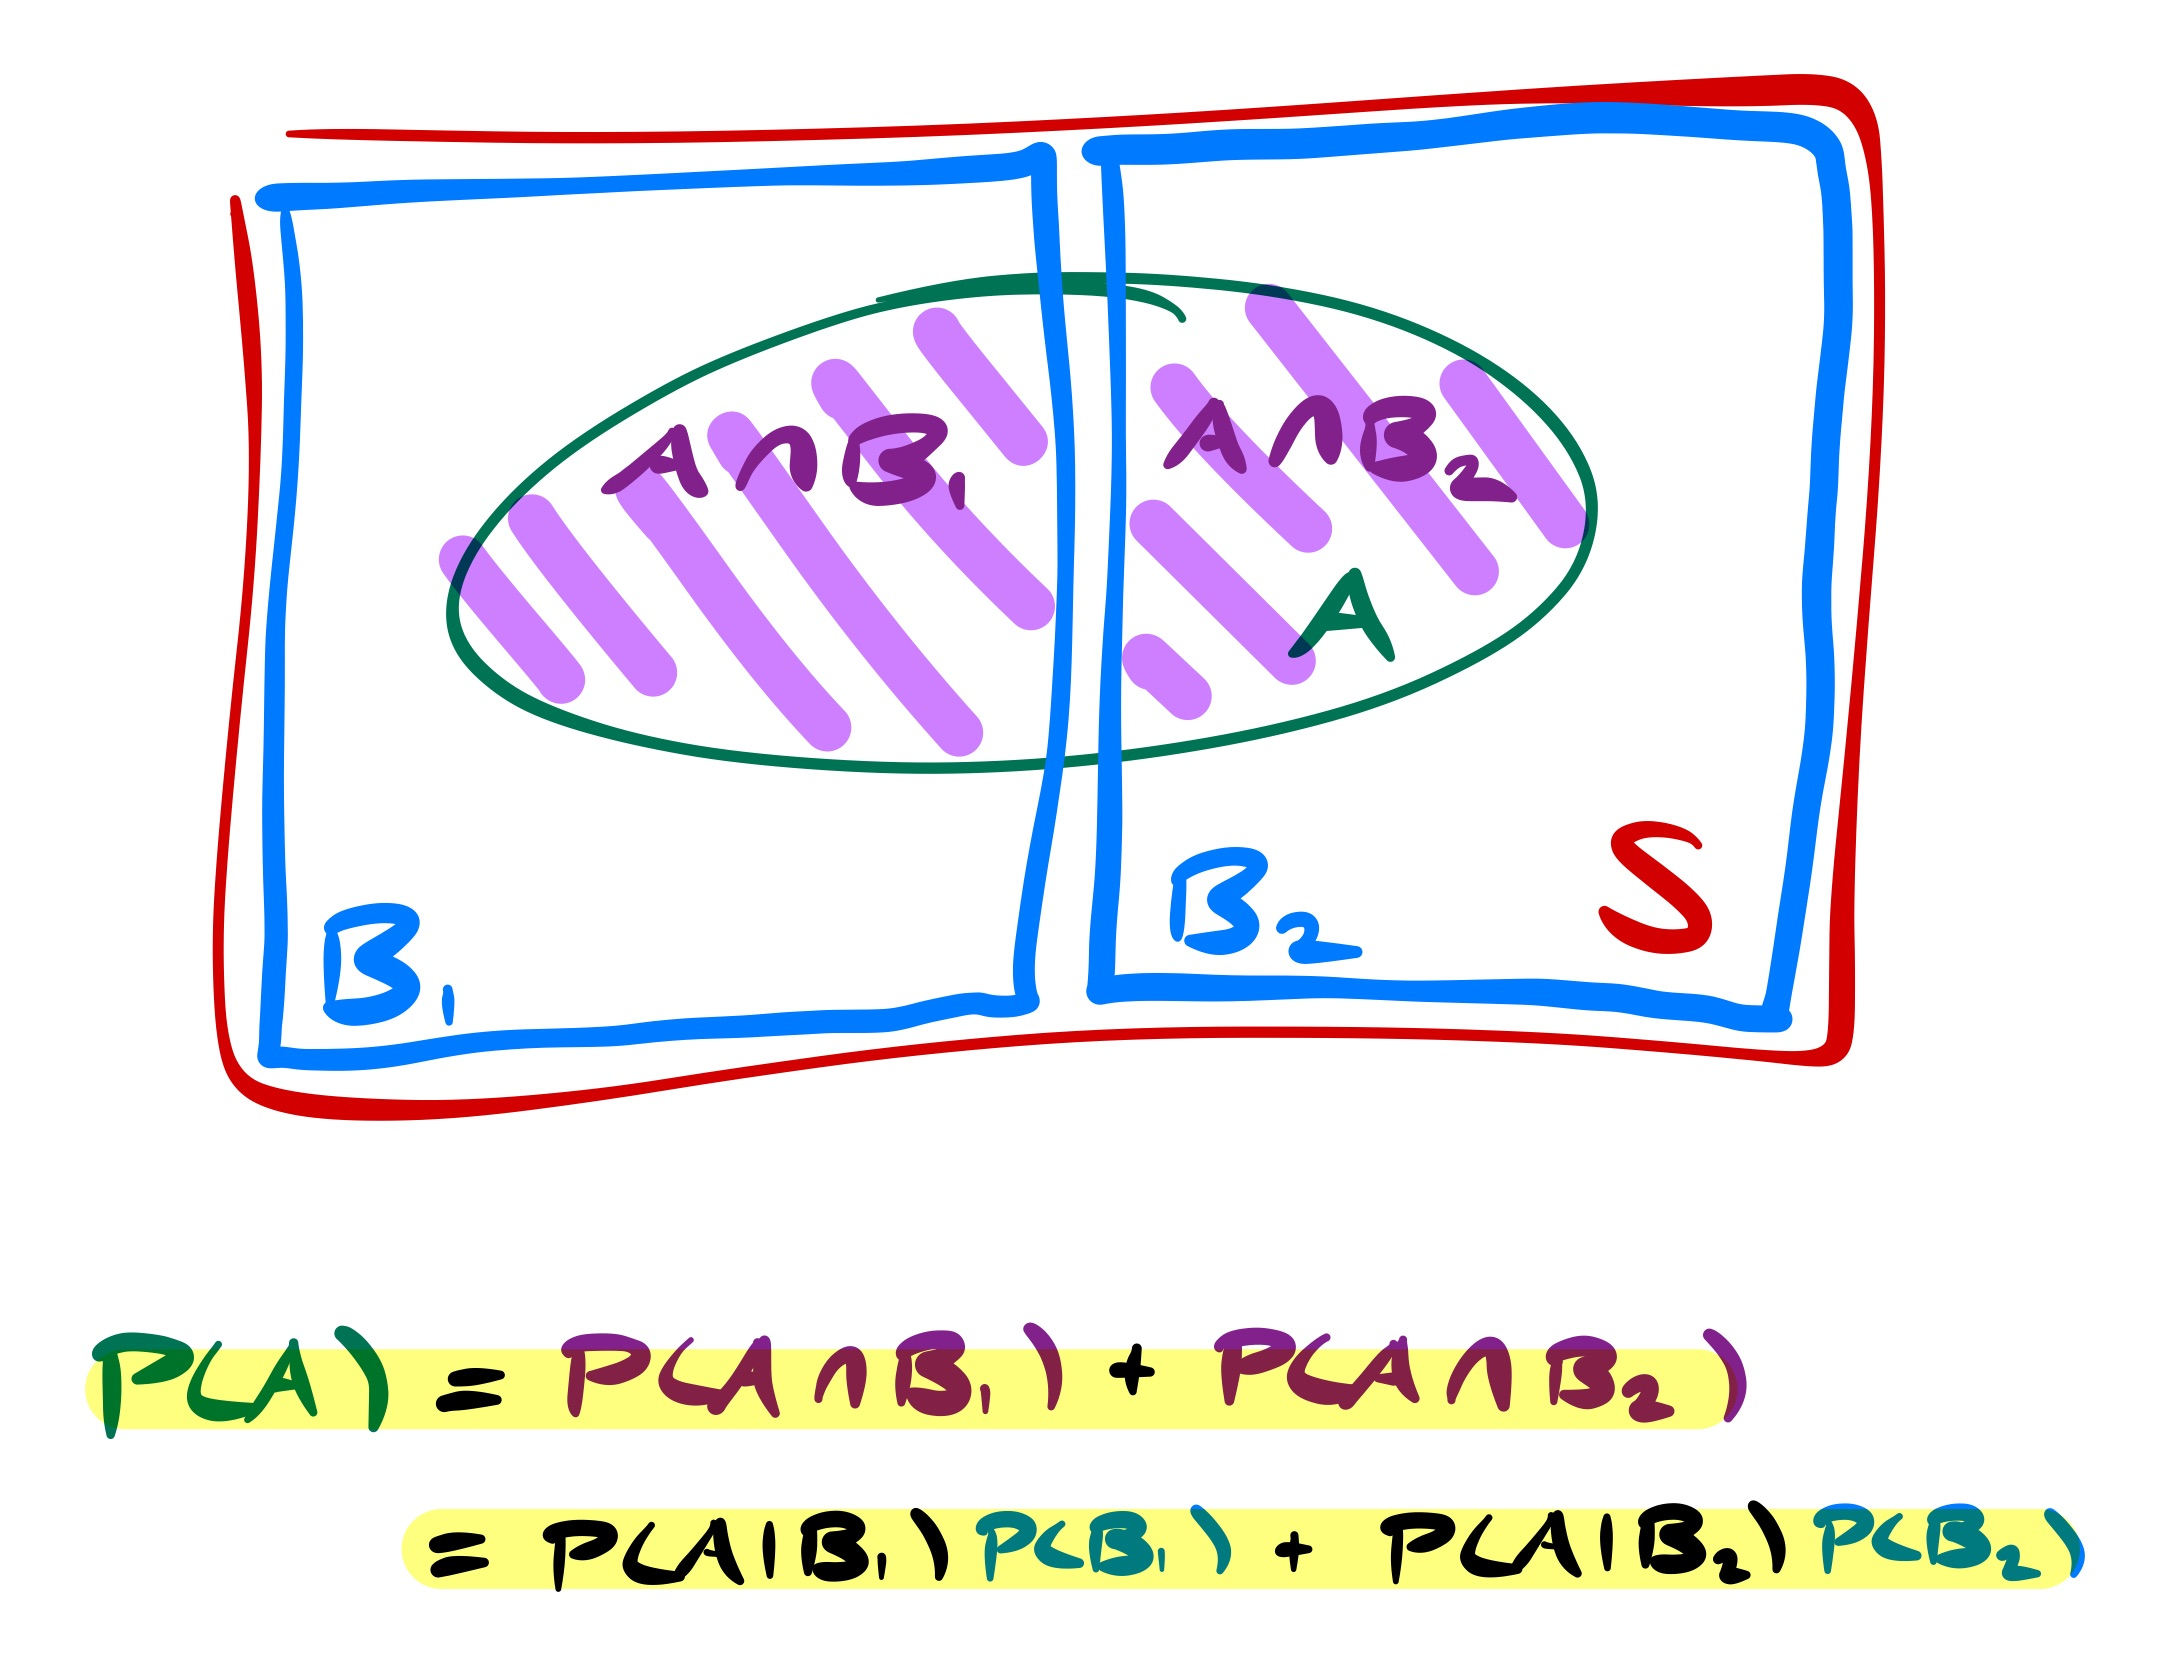
\includegraphics[width=0.5\textwidth]{stat110_section2_figure4.jpg}\\
  {\footnotesize FIGURE 4: The sample space partitioned by $B_1$ and $B_2$ illustrating LOTP for 2 events.}
\end{center}

\begin{definition}[Partition]
Events $B_1, \ldots, B_n$ \textit{partition} the sample space if each \textit{pairwise intersection} is empty and their \textit{union} is the entire sample space.

$\bullet$ Mathematically, $B_i \cap B_j = \emptyset$ for all $i \neq j$ and $\bigcup_{i = 1}^{n} B_i = S$ such that $\sum_{i = 1}^{n} P(B_i) = 1$.
\end{definition}

\begin{definition}[Law of Total Probability (LOTP)]
\[P(A) = \sum_{i = 1}^{n} P(A \mid B_i) P(B_i),\] where $B_1, \ldots, B_n$ partition the sample space.

$\bullet$ Since $B_1, \ldots, B_n$ partition the sample space, $P(A) = P(A \cap B_1) + \ldots + P(A \cap B_n)$, and $P(A \cap B_i) = P(A \mid B_i) P(B_i)$. This is illustrated in Figure 4.

$\bullet$ \tip LOTP is useful when we want to condition on something (i.e., \enquote{wishful thinking}). Also, LOTP is useful to find the denominator in Bayes' Rule.
\end{definition}

\begin{concept}
Suppose that every upperclassman has a probability $p$ of owning a scooter. If they live in the Quad, $p = \frac{1}{10}$. Otherwise, $p = \frac{1}{20}$. What is the probability that a randomly selected upperclassman owns a scooter?
\end{concept}

\begin{solutionbox}
Let $S$ be the event that they own a scooter and $Q$ be the event that they’re in the Quad. Notice the wishful thinking, where we really want to know whether they're in the Quad or not.

\[
\begin{aligned}
P(S) &= P(S \mid Q) P(Q) + P(S \mid Q^c) P(Q^c) && \text{by LOTP} \\
&= (1/10)(3/12) + (1/20)(9/12) && \text{since $p = \frac{1}{10}$ for the 3 Quad houses} \\
&= 0.0625 && \text{by simplifying}
\end{aligned}
\]

Notice $P(S) = 0.0625$ is weighted toward $p = \frac{1}{20}$, which makes sense since the majority of students don't live in the Quad and thus have a lower probability of owning a scooter.
\end{solutionbox}

% Section: Disjoint and Independent Events
\section{Disjoint and Independent Events}

\begin{idea}
Different events are often related to each other, whether by being \textit{disjoint} or \textit{independent}. Importantly, things get more complicated with three (or more) events.
\end{idea}

\begin{definition}[Disjointness]
Events $A$ and $B$ are \textit{disjoint} if they cannot happen simultaneously.

$\bullet$ Mathematically, $P(A \cap B) = 0$.
\end{definition}

\begin{definition}[Independence]
Events $A$ and $B$ are \textit{independent}, denoted $A \indep B$, if knowing one gives no information about the other.

$\bullet$ Mathematically, $P(A \mid B) = P(A)$ and $P(B \mid A) = P(B)$, which imply $P(A \cap B) = P(A) P(B)$.

$\bullet$ If $A \indep B$, then $A^c \indep B$, $A^c \indep B^c$, and $A \indep B^c$.
\end{definition}

\begin{definition}[Independence of three events]
Events $A$, $B$, and $C$ are \textit{independent} if $P(A \cap B) = P(A) P(B)$, $P(A \cap C) = P(A) P(C)$, $P(B \cap C) = P(B) P(C)$, and $P(A \cap B \cap C) = P(A) P(B) P(C)$.

$\bullet$ If only the first three conditions hold, then $A$, $B$, and $C$ are \textit{pairwise independent}, but the last condition is needed for $A$, $B$, and $C$ to be \textit{independent}.
\end{definition}

\begin{definition}[Conditional independence]
Events $A$ and $B$ are \textit{conditionally independent given $C$}, denoted $(A \indep B) \mid C$, if, conditional on $C$, knowing one gives no information about the other.

$\bullet$ Mathematically, $P(A \mid B, C) = P(A \mid C)$ and $P(B \mid A, C) = P(B \mid C)$, which imply $P(A \cap B \mid C) = P(A \mid C) P(B \mid C)$. Notice this takes the definition of (unconditional) independence and adds \enquote{$\mid C$} to everything.

$\bullet$ \warning Conditional independence does \textit{not} imply (unconditional) independence, and vice versa.
\end{definition}

\begin{example}[Unconditional independence]
I have two fair $6$-sided dice, so the rolls are \textit{independent} (e.g., if I roll a $6$ on the first one, I still don't know what I'll get on the next one). But if we condition on the event that the sum is $10$, the second roll is deterministic from the first one and thus \textit{not conditionally independent}.

$\bullet$ Mathematically, let $X_i$ be the value of my $i$th roll. $\{X_1 = 6\} \indep \{X_2 = 4\}$, but $(\{X_1 = 6\} \notindep \{X_2 = 4\}) \mid \{X_1 + X_2 = 10\}$.
\end{example}

\begin{example}[Conditional independence]
Let $p$ be the probability I make a free throw. If I shoot $9$ free throws that all miss, you'd probably assume that the $10$th shot would miss because the event that I miss $9$ shots implies that $p$ is low. But if we condition on $p = 0.5$, then the $10$th shot is \textit{conditionally independent} of the previous $9$; I'm just having an unlucky day.

$\bullet$ Mathematically, let $A$ be the event that I miss the first $9$ shots and $B$ be the event that I miss the $10$th shot. $A \notindep B$, but $(A \indep B) \mid \{p = 0.5\}$.
\end{example}

% Section: Extensions of Bayes' Rule and LOTP
\section{Extensions of Bayes' Rule and LOTP}

\begin{idea}
When working with three events, we can extend our previous tools using two main tricks: extra conditioning, and treating an intersection as one event.
\end{idea}

\begin{definition}[Bayes' Rule with extra conditioning]
\[P(A \mid B, C) = \frac{P(B \mid A, C) P(A \mid C)}{P(B \mid C)},\] where $P(B \mid C) > 0$.

$\bullet$ Notice that this takes \enquote{regular} Bayes' Rule—i.e., $P(A \mid B) = \frac{P(B \mid A) P(A)}{P(B)}$—and adds \enquote{$\mid C$} to everything.
\end{definition}

\begin{definition}[Bayes' Rule with $B, C$ as one event]
\[P(A \mid B, C) = \frac{P(B, C \mid A) P(A)}{P(B, C)},\] where $P(B, C) > 0$.

$\bullet$ Notice that this takes \enquote{regular} Bayes' Rule—i.e., $P(A \mid B) = \frac{P(B \mid A) P(A)}{P(B)}$—and replaces $B$ with $B, C$.
\end{definition}

\begin{definition}[LOTP with extra conditioning]
\[P(A \mid C) = \sum_{i = 1}^{n} P(A \mid B_i, C) P(B_i \mid C),\] where $B_1, \ldots, B_n$ partition the sample space.

$\bullet$ Notice that this takes \enquote{regular} LOTP—i.e., $P(A) = \sum_{i = 1}^{n} P(A \mid B_i) P(B_i)$—and adds \enquote{$\mid C$} to everything.
\end{definition}

\begin{concept}
Bayes' Rule with extra conditioning requires that $P(B \mid C) > 0$, and Bayes' Rule with $B, C$ as one event requires that $P(B, C) > 0$. Why are these the same condition?
\end{concept}

\begin{solutionbox}
$P(B \mid C) > 0 \implies P(B, C) > 0$ since $P(B \mid C) = \frac{P(B, C)}{P(C)}$, and $P(B, C) > 0 \implies P(B \mid C) > 0$ since $P(B, C) = P(C) P(B \mid C)$. Thus, $P(B \mid C) > 0 \iff P(B, C) > 0$.
\end{solutionbox}

% Section: Recap
\section{Recap}

\begin{idea}
Let's review the main rules and strategies we've discussed for calculating probability.
\end{idea}

\begin{definition}[Probability toolkit]
Informally, \textit{probability} is a measure of how likely an event is, bounded from $0$ to $1$.

$\bullet$ $P(A) = \frac{\text{\# of outcomes favorable to $A$}}{\text{\# of total outcomes in $S$}} = \frac{|A|}{|S|}$ by Naive Probability, where the sample space is finite and consists of equally likely outcomes.

$\bullet$ $P(A) \leq P(B)$ if $A$ implies $B$. 

$\bullet$ $P(A \cup B) = P(A) + P(B) - P(A \cap B)$ by PIE.

$\bullet$ $P(A \cap B) = P(A, B) = P(A) P(B \mid A) = P(B) P(A \mid B)$ by Multiplication Rule.

$\bullet$ $P(A) = 1 - P(A^c)$ by Complement Rule.

$\bullet$ $P((A \cup B)^c) = P(A^c \cap B^c)$, $P((A \cap B)^c) = P(A^c \cup B^c)$ by De Morgan's Laws.

$\bullet$ $P(A) = \sum_{i = 1}^{n} P(A \cap B_i) = \sum_{i = 1}^{n} P(A \mid B_i) P(B_i)$ by LOTP, where $B_1, \ldots, B_n$ partition the sample space.

$\bullet$ $P(A \mid B) = \frac{P(A \cap B)}{P(B)} = \frac{P(B \mid A) P(A)}{P(B)}$ by Bayes' Rule.

$\bullet$ $P(A \mid C) = \sum_{i = 1}^{n} P(A \cap B_i \mid C) = \sum_{i = 1}^{n} P(A \mid B_i, C) P(B_i \mid C)$ by LOTP with Extra Conditioning, where $B_1, \ldots, B_n$ partition the sample space.

$\bullet$ $P(A \mid B, C) = \frac{P(A \cap B \mid C)}{P(B \mid C)} = \frac{P(B \mid A, C) P(A \mid C)}{P(B \mid C)}$ by Bayes' Rule with Extra Conditioning.

$\bullet$ $P(A \mid B, C) = \frac{P(A \cap B, C)}{P(B, C)} = \frac{P(B, C \mid A) P(A)}{P(B, C)}$ by Bayes' Rule with $B, C$ as One Event.

$\bullet$ \tip The complement is useful for finding the event of \enquote{at least} something.

$\bullet$ \tip We can treat $A \cap B$ (or any union or intersection) as \textit{one} event!

$\bullet$ \tip All conditional probabilities \textit{are} probabilities, and all probabilities \textit{are} conditional probabilities (implicitly conditioning on $S$).

$\bullet$ \tip Often, we want to find $P(A \mid B)$ but are given $P(B \mid A)$. This is where Bayes' Rule is useful!

$\bullet$ \tip LOTP is useful when we want to condition on something (i.e., \enquote{wishful thinking}). Also, LOTP is useful to find the denominator in Bayes' Rule.
\end{definition}

% Section: Exercises
\section{Exercises}

\begin{problem}
Suppose that we're on the game show \textit{Let's Make a Deal} hosted by Monty Hall. We choose 1 of the 3 closed doors, 2 of which have a goat behind them and 1 of which has a car. Monty, who knows where the car is, then opens 1 of the 2 remaining doors. The door he opens always has a goat behind it (i.e., he never reveals the car). If he has a choice, he picks a door at random with equal probabilities. Monty then offers us the option of switching to the other unopened door. If our goal is to get the car, should we switch doors?\footnote{Inspired by Example 2.7.1 in \textit{Introduction to Probability} by Joseph K. Blitzstein and Jessica Hwang and Problem 1 in \enquote{Stat 110 Homework 3, Fall 2024} by Joseph K. Blitzstein.}

(a) Find the probability that we win the car if we don't switch doors.

(b) Find the probability that we win the car if we switch doors.

(c) Now suppose that Monty is a very old man and his memory isn’t as good as it used to be. With probability $p$, he remembers where the car is, and the game proceeds as usual. But with probability $q = 1 - p$, he forgets where the car is, in which case he chooses randomly, with equal probabilities, which door (other than our initial choice) to open. It’s possible that he reveals the car, which would spoil the game. If the game is spoiled, Monty apologizes, and we get nothing. Find the probability that we win the car if we switch doors.
\end{problem}

\begin{solutionbox}
(a) It's random which of the 3 doors has the car, so by the naive definition of probability, our initial guess has a success probability of $\frac{1}{3}$.

(b) Let's label the doors 1 through 3. Without loss of generality, assume we picked door 1. (If you don't want to pick door 1, we could simply relabel the doors.) Let $A$ be the event that we win the car, and let $C_i$ be the event that the car is behind door $i$. By LOTP, $P(A) = P(A \mid C_1) \times \frac{1}{3} + P(A \mid C_2) \times \frac{1}{3} + P(A \mid C_3) \times \frac{1}{3}$. If the car is behind door 1, switching will fail. If the car is behind door 2 or door 3, switching will succeed (since the remaining unopened door must contain the car if Monty always reveals a goat). Thus, $P(A) = 0 \times \frac{1}{3} + 1 \times \frac{1}{3} + 1 \times \frac{1}{3} = \frac{2}{3}$. We should switch doors!

(c) We'll use the same notation as above. Let $R$ be the event that Monty remembers where the car is. By LOTP, $P(A) = P(A \mid R) P(R) + P(A \mid R^c) P(R^c)$. Given $R$, the game proceeds as usual, so $P(A \mid R) = \frac{2}{3}$. But given $R^c$, we win the car if and only if the car is not behind our initial guess (like before) AND Monty doesn't spoil the game (which he would do with probability $\frac{1}{2}$). Thus, $P(A) = \frac{2}{3} \times p + \left( \frac{2}{3} \right) \left( \frac{1}{2} \right) \times q = \frac{p + 1}{3}$. Notice that if $p = 1$ (i.e., he never forgets), this reduces to our previous answer.
\end{solutionbox}

\begin{problem}
There are 2 different diseases that cause a certain weird symptom, and anyone who has either or both of these diseases will experience the symptom. Let $D_1$ be the event of having the first disease, $D_2$ be the event of having the second disease, and $W$ be the event of having the weird symptom. Suppose that $D_1$ and $D_2$ are independent, with $P(D_j) = p_j$, and a person with neither of these diseases will have the weird symptom with probability $w_0$. Let $q_j = 1 - p_j$, and assume that $0 < p_j < 1$.\footnote{Inspired by Problem 1 in \enquote{Stat 110 Final from 2016} by Joseph K. Blitzstein.}

(a) Find $P(W)$.

(b) Find $P(D_1 \mid W)$ and $P(D_1, D_2 \mid W)$.
\end{problem}

\begin{solutionbox}
(a) Let $D = D_1 \cup D_2$ (i.e., the event of having either of these diseases).

\[
\begin{aligned}
P(W) &= P(W \mid D) P(D) + P(W \mid D^c) P(D^c) && \text{by LOTP} \\
&= 1 \times P(D) + w_0 \times P(D^c) && \text{by substituting} \\
&= P(D_1 \cup D_2) + w_0 \times P(D_1^c, D_2^c) && \text{by De Morgan's Laws} \\
&= P(D_1) + P(D_2) - P(D_1, D_2) + w_0 \times P(D_1^c) P(D_2^c) && \text{by PIE and independence} \\
&= p_1 + p_2 - p_1 p_2 + w_0 \times q_1 q_2 && \text{by substituting} \\
&= 1 - (1 - w_0) q_1 q_2 && \text{by simplifying}
\end{aligned}
\]

(b) We'll use the same notation as above.

\[
\begin{aligned}
P(D_1 \mid W) &= \frac{P(W \mid D_1) P(D_1)}{P(W)} && \text{by Bayes' Rule} \\
&= \frac{1 \times p_1}{P(W)} && \text{by substituting} \\
&= \frac{p_1}{1 - (1 - w_0) q_1 q_2} && \text{from (a)}
\end{aligned}
\]

\[
\begin{aligned}
P(D_1, D_2 \mid W) &= \frac{P(W \mid D_1, D_2) P(D_1, D_2)}{P(W)} && \text{by Bayes' Rule} \\
&= \frac{P(W \mid D_1, D_2) P(D_1) P(D_2)}{P(W)} && \text{by independence} \\
&= \frac{1 \times p_1 p_2}{P(W)} && \text{by substituting} \\
&= \frac{p_1 p_2}{1 - (1 - w_0) q_1 q_2} && \text{from (a)}
\end{aligned}
\]
\end{solutionbox}

\begin{problem}
Let $r$ be the probability that a student in a class reads the textbook, with $0 < r < 1$. Suppose that solving a certain problem correctly is twice as likely for someone who has read the textbook compared to someone who has not.\footnote{Inspired by Problem 3 in \enquote{Stat 110 Homework 2, Fall 2024} by Joseph K. Blitzstein.}
 
(a) Find the probability that a student read the textbook, given they solved the problem correctly.
\end{problem}

\begin{solutionbox}
Let $C$ be the event that someone solves the problem correctly and $R$ be the event that someone reads the textbook. Let $x = P(C \mid R) = 2 P(C \mid R^c)$.

\[
\begin{aligned}
P(R \mid C) &= \frac{P(C \mid R) P(R)}{P(C)} && \text{by Bayes' Rule} \\
&= \frac{P(C \mid R) P(R)}{P(C \mid R) P(R) + P(C \mid R^c) P(R^c)} && \text{by LOTP} \\
&= \frac{x \times r}{x \times r + \frac{x}{2} \times (1 - r)} && \text{by substituting} \\
&= \frac{2r}{r + 1} && \text{by simplifying}
\end{aligned}
\]
\end{solutionbox}

\end{document}